\subsection{Adaptive photoreceptor}

Since biological photoreceptors are adaptive and amplifiy changes more than static inputs, a silicon photoreceptor that mimics this by providing a low gain for DC but a high gain for AC is the adaptive photoreceptor circuit given in \ref{fig:AdaptivePhotoreceptor1}.

\begin{figure}[H]
    \centering
    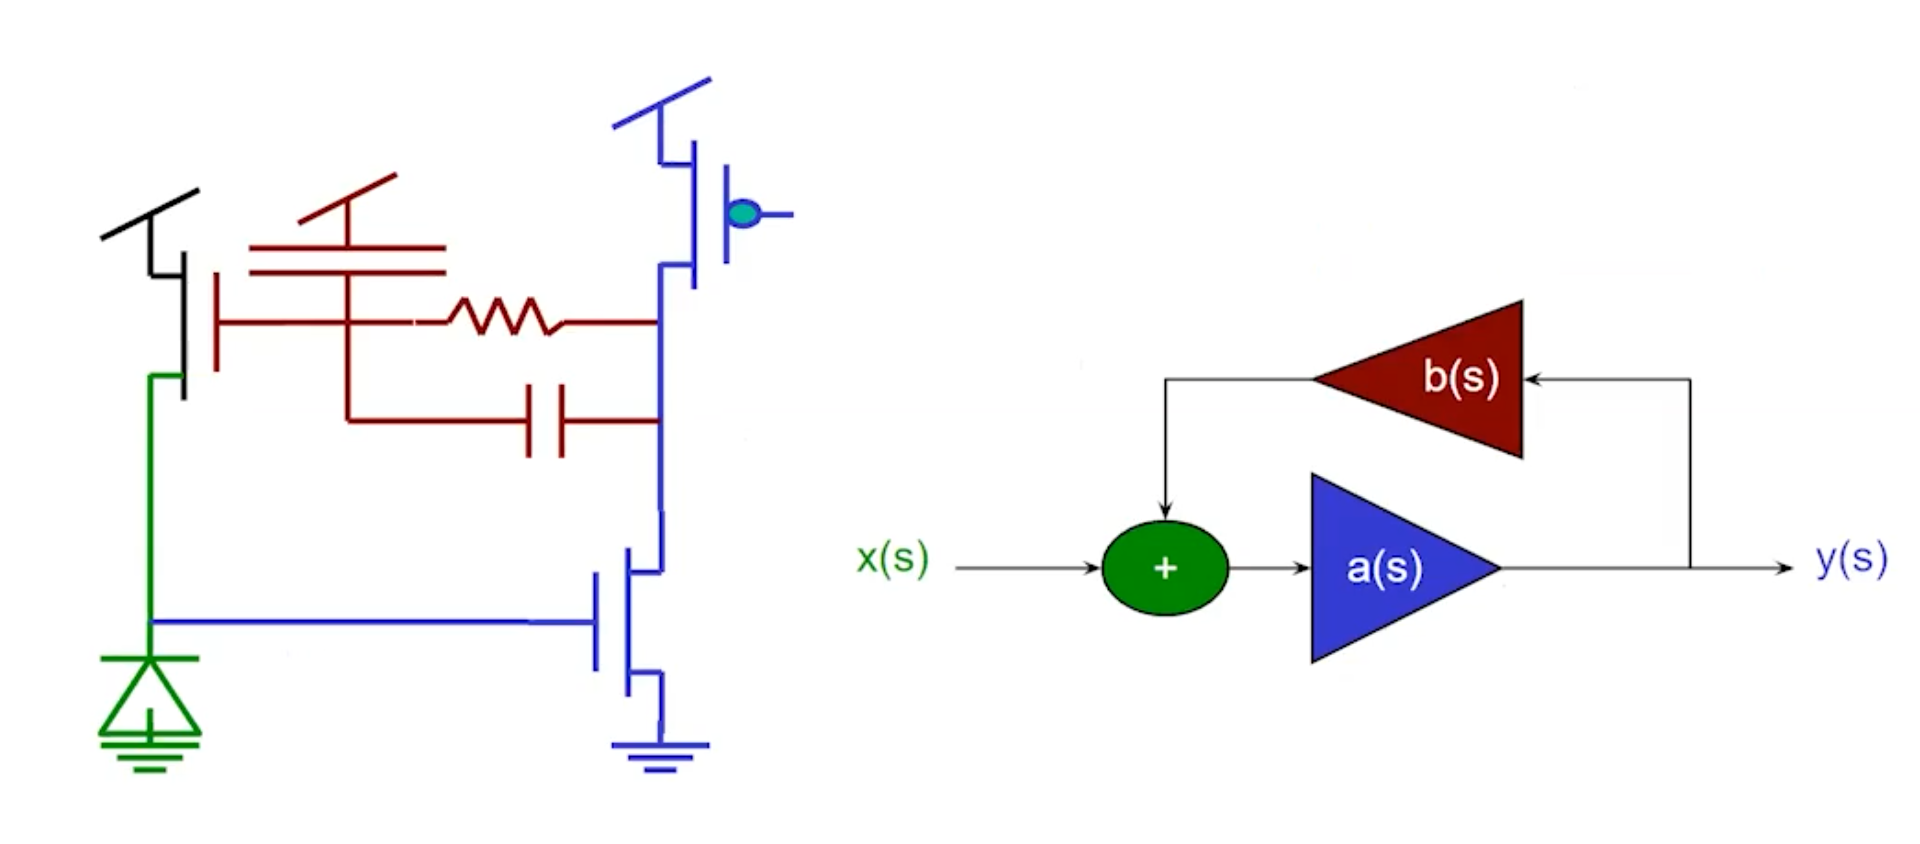
\includegraphics[width=1\linewidth]{../../Figures/adaptive_photoreceptor.png}
    \caption{Adaptive photoreceptor, as shown in the lecture slides.}
    \label{fig:AdaptivePhotoreceptor1}
\end{figure}

\begin{figure}[H]
    \centering
    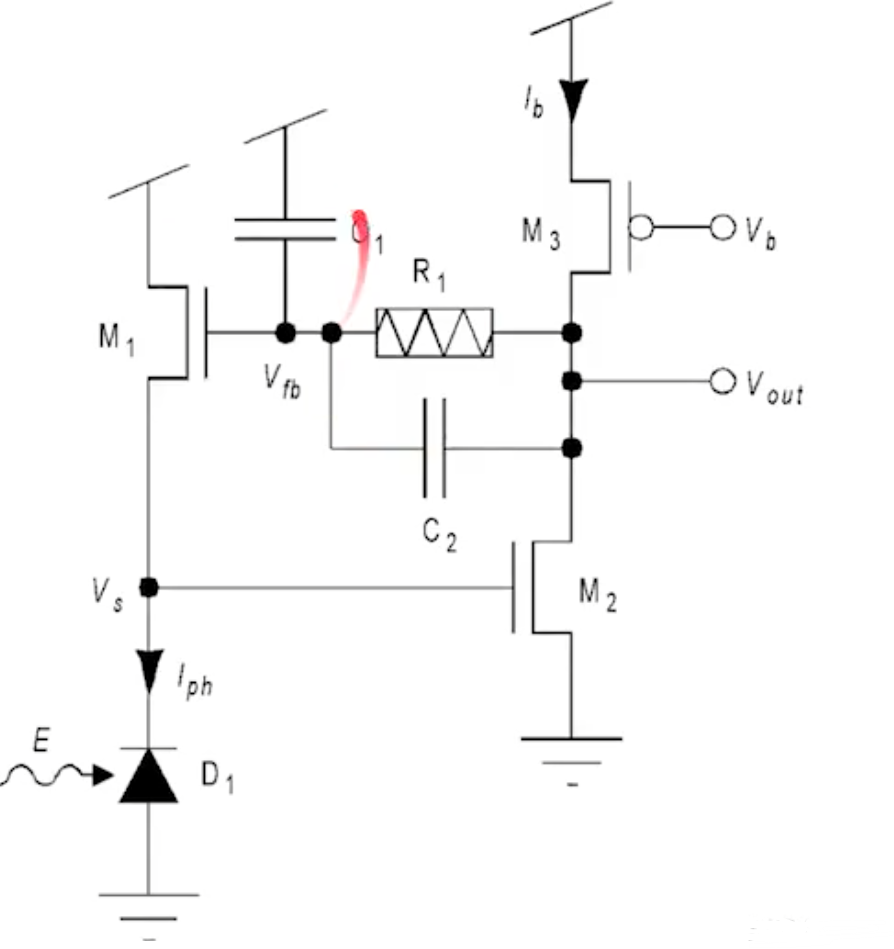
\includegraphics[width=1\linewidth]{../../Figures/adaptive_photoreceptor2.png}
    \caption{Adaptive photoreceptor in detail.}
    \label{fig:AdaptivePhotoreceptor2}
\end{figure}